\section{Related Work}
\label{sec:related}

\begin{figure*}[t]
    \centering
    \addtolength{\tabcolsep}{-4pt}
    \begin{tabular}{cccccc}
		\begin{overpic}[width=0.16\textwidth]{images/validations/compare1/plane_fullsim_ref_3_2h.jpg} 
    		%\put(2,3){\bfseries \color{white} \Large } 
    	\end{overpic} &
		\begin{overpic}[width=0.16\textwidth]{images/validations/compare1/plane_10s_pt_98spp.jpg} 
		\put(2,3){\bfseries \color{white} 98 spp} 
		\end{overpic} &
		\begin{overpic}[width=0.16\textwidth]{images/validations/compare1/plane_10s_bdpt_35spp.jpg} 
		\put(2,3){\bfseries \color{white} 35 spp} 
		\end{overpic} &
		\begin{overpic}[width=0.16\textwidth]{images/validations/compare1/plane_10s_mlt_280spp.jpg}
		\put(2,3){\bfseries \color{white} 280 spp} 
		\end{overpic} &
		\begin{overpic}[width=0.16\textwidth]{images/validations/compare1/plane_10s_uni_56spp.jpg} 
		\put(2,3){\bfseries \color{white} 56 spp} 
		\end{overpic} &
		\begin{overpic}[width=0.16\textwidth]{images/validations/compare1/plane_10s_bi_26spp.jpg} 
		\put(2,3){\bfseries \color{white} 26 spp} 
		\end{overpic}
		\\
		\begin{overpic}[width=0.16\textwidth]{images/validations/compare1/plane_fullsim_ref_4_8h.jpg} 
			%\put(2,3){\bfseries \color{white} \Large } 
		\end{overpic} &
		\begin{overpic}[width=0.16\textwidth]{images/validations/compare1/plane_10s_pt_60spp.jpg} 
		\put(2,3){\bfseries \color{white} 60 spp} 
		\end{overpic} &
		\begin{overpic}[width=0.16\textwidth]{images/validations/compare1/plane_10s_bdpt_25spp.jpg} 
		\put(2,3){\bfseries \color{white} 25 spp} 
		\end{overpic} &
		\begin{overpic}[width=0.16\textwidth]{images/validations/compare1/plane_10s_mlt_80spp.jpg} 
		\put(2,3){\bfseries \color{white} 80 spp} 
		\end{overpic} &
		\begin{overpic}[width=0.16\textwidth]{images/validations/compare1/plane_10s_uni_15spp.jpg} 
		\put(2,3){\bfseries \color{white} 15 spp} 
		\end{overpic} &
		\begin{overpic}[width=0.16\textwidth]{images/validations/compare1/plane_10s_bi_19spp.jpg} 
		\put(2,3){\bfseries \color{white} 19 spp} 
		\end{overpic}
		\\
		%
		Reference &
		Standard PT &
		Standard BDPT &
		Standard MLT &
		Our unidirectional &
		Our bidirectional
	\end{tabular}
    \caption{\label{fig:validation1}
    	\textbf{Equal-time comparisons} of our unidirectional and bidirectional approach to standard transport algorithms, on a simple flat layered configuration lit by a small area light. 
    	\sz{For standard PT, BDPT and MLT, results are all generated using 3D tracing by applying these algorithms in a simple 3D scene containing a very large slab with flat interfaces.} 
    	%Again, performance is dominated by shading computation, as the scene is trivial.
    	\textbf{Top}: A single slab with Henyey-Greenstein scattering between two interfaces, where our estimators perform similarly, but both significantly outperform path tracing, bidirectional and Metropolis transport. \textbf{Bottom}: A more complex configuration with two slabs and three interfaces; both media are using an anisotropic microflake phase function \cite{Jakob:2010:RTF}. Our bidirectional estimator is a clear winner in this case.
    	\sz{The references are generated using standard PT with 100K spp, and all the other images are rendered in 10 seconds.}
    }
\end{figure*}

\subsection{Discretized layered BSDFs}
%\myparagraph{Discretized layered BSDFs}
Previously, a number of BSDF models have been proposed to describe layers with various assumptions on the interface and subsurface scattering.

An early analytical model by Hanrahan and Krueger \shortcite{Hanrahan1993} already supported multiple layers, but only single scattering, and without supporting arbitrary BSDFs at interfaces. They also proposed to add multiple scattering by Monte Carlo simulation, but their simulation approach only considers volume scattering events (as opposed to a combination of volume and rough interface events). Furthermore, it uses binning on the outgoing direction, as opposed to an efficient BSDF evaluation method for a given outgoing direction, which is provided by our approach.

A model by Stam \shortcite{Stam2001} introduces a solution for rendering skin as a layered material consisting of rough dielectric interfaces bounding a volumetric scattering slab. The solution is based on discretization of the BSDF into a directional basis, on which the light transport problem is solved. The model introduced by Jakob~et~al.~\shortcite{Jakob:2014:CFR} can be seen as a significant extension of Stam's discretization approach, working in the Fourier domain. It handles arbitrary layer stacks, supporting subsurface scattering within thin layers using the adding-doubling method, in addition to microfacet rough interfaces. The work of Zeltner extends this approach to anisotropic surface reflectance \shortcite{Zeltner2018}. These models are highly accurate and efficient to render with, once the discretized BSDF has been constructed. However, as the BSDF construction in the discretized basis is relatively expensive, they are best suited for homogeneous BSDFs. A small number of such BSDFs can be spatially blended with varying weights, but this has strict limitations, compared to our support for arbitrary spatial texturing of all parameters.

\subsection{Analytic layered BSDFs}
%\myparagraph{Approximate layered BSDFs}
The model by Weidlich and Wilkie \shortcite{Weidlich:2007:ALM} takes a different approach. They focus on layers where subsurface scattering is absent (though absorption is allowed), by analytically combining microfacet BSDFs from the interfaces into a single, potentially multi-lobe, microfacet-like BSDF. There are significant approximations in this approach, carefully chosen so that integration (Monte Carlo or otherwise) is never required within a single BSDF query. This makes the model fast and flexible. Another recent model \cite{guo2017rendering} also takes the approach of avoiding Monte Carlo integration during queries, by introducing extended normal distribution functions (ENDFs), analogous to microfacet NDFs but capturing multiple reflection or scattering events. In the most recent work, Belcour \shortcite{Belcour2018} introduced an approach based on tracking low-order moments of the BSDF lobes. This is a very fast and practical solution, but still introduces some approximations and limitations (e.g. no surface or volume anisotropy). In contrast, our method offers unbiased accuracy and even more flexibility, at the cost of some additional computation and variance. \sz{Several previous techniques model light scattering in layered materials like human skin~\cite{Donner:2008:LHR}, but these are focused on lateral light spreading in BSSRDFs, and are orthogonal to our focus on the directional properties of BSDF models.}

\subsection{Microfacet models for interfaces}
%\myparagraph{Microfacet models for interfaces}
BSDF models based on the microfacet theory are commonly used in computer graphics to capture how light reflects and refracts when interacting with specular surfaces with rough microstructure. The model by Walter~et~al.~\shortcite{Walter:2007:MMR} extends the microfacet model of Cook and Torrance~\shortcite{Cook:1982:RMC} to handle light reflection and transmittance through rough dielectric interfaces, and is currently seen as standard in physically-based rendering. We use this model to describe our layer interfaces.

The microfacet model recently developed by Heitz~et~al.~\shortcite{Heitz:2016:MMB} is capable of capturing interreflections between the facets and better conserves energy. Sch\"ussler \shortcite{Schussler2017} introduced a solution to the energy loss common in normal mapping techniques, caused by a mismatch between the shading and geometric normal. These models (or any future improved microfacet models) could be combined with our approach.

\subsection{Capability comparison}
%\myparagraph{Capability comparison}
In Figure \ref{fig:compare-previous}, we compare the capabilities of our approach to recent work \cite{Zeltner2018,Belcour2018}. We consider three features supported by our approach: surface anisotropy, spatial variation, and volumetric medium anisotropy. Only one of these is supported in the compared systems: spatial variation in Belcour's approach and surface anisotropy in Zeltner's.

% comparison figure (Zeltner / Belcour)
\begin{figure}[t]
	\addtolength{\tabcolsep}{-3pt}
	\begin{tabular}{ccc}
	    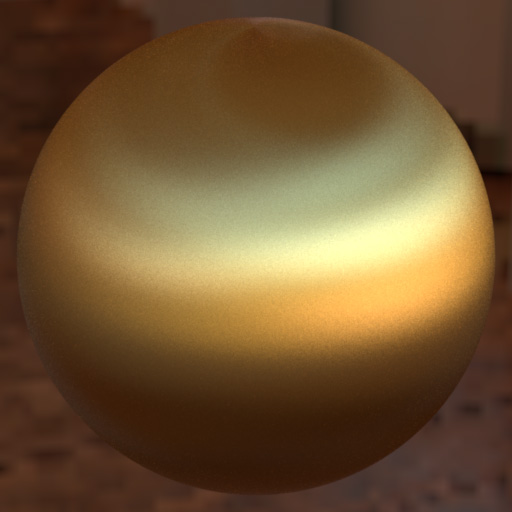
\includegraphics[width=0.315\columnwidth]{images/validations/compare2/aniso_comb_hor_hor_512spp_17min.jpg} &
	    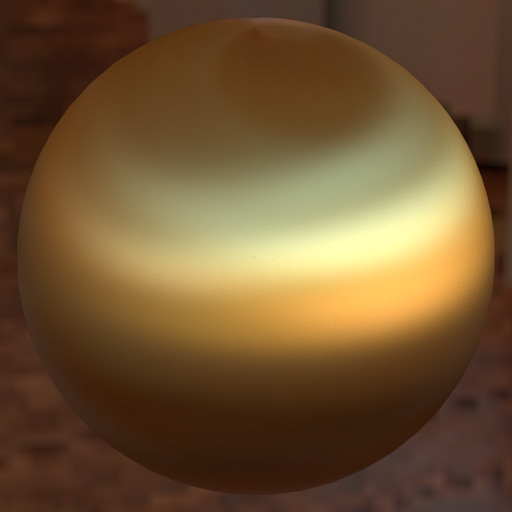
\includegraphics[width=0.315\columnwidth]{images/validations/compare2/aniso_comb_hor_hor_wenzel.jpg} &
	    
\includegraphics[width=0.315\columnwidth]{images/validations/compare2/na.pdf} \\

	    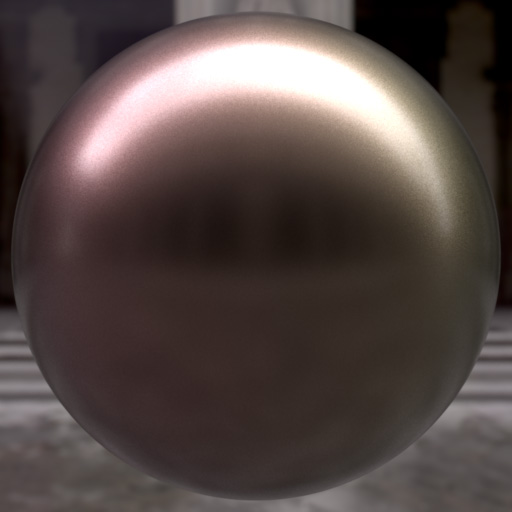
\includegraphics[width=0.315\columnwidth]{images/validations/compare2/sphere_layered_1024spp_37min.jpg} &
	    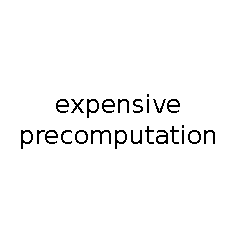
\includegraphics[width=0.315\columnwidth]{images/validations/compare2/na2.pdf} &
	    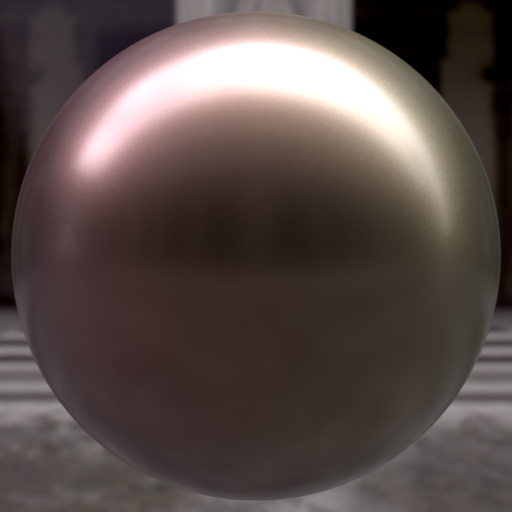
\includegraphics[width=0.315\columnwidth]{images/validations/compare2/sphere_laurent_1024spp_1_5min.jpg} \\

	    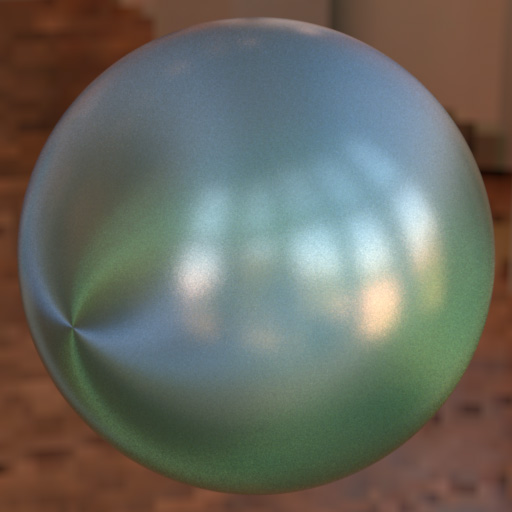
\includegraphics[width=0.315\columnwidth]{images/validations/compare2/sphere_1024spp_60min.jpg} &
	    
\includegraphics[width=0.315\columnwidth]{images/validations/compare2/na.pdf} &
	    
\includegraphics[width=0.315\columnwidth]{images/validations/compare2/na.pdf} \\

	    Ours &
	    [Zeltner 2018] &
	    \cite{Belcour2018}
	\end{tabular}
	%
    \caption{\label{fig:compare-previous}
    	\textbf{Comparison to previous work.} The \textbf{top row} shows an example with anisotropic surface reflectance, where our solution closely matches Zeltner's, but Belcour's approach does not support anisotropy. The \textbf{middle row} shows an example with spatial variation in the parameters; here our method closely matches Belcour's, but Zeltner's approach does not naturally support spatial variation. The \textbf{bottom row} shows a two-layer configuration with anisotropic microflake phase functions, which is only supported by our method.
    }
\end{figure}

%\sz{
%\myparagraph{Specialized models}
%Previously, a few specialized techniques have been developed to model light scattering in materials like human skin~\cite{Donner:2008:LHR} and clouds~\cite{bouthors2006real,sekiguchi2017simple}.
%These methods are largely orthogonal to this work as they focus on light transport problems with very different settings.
%}

